\chapter{HDSS Sites Visualization Platform }
\label{methods}

\textit{This chapter gives a description of the the scope of the research, and overview of the solution, including a discussion on the three themes of Scientific Portal, Data Operations Portal and Community Engagement Portal. It goes on to describe in detail how the the application which serve the three themes were constructed, in terms of the tools, programming platforms and languages as well as relevant algorithms to replicate key artefacts.}
\vspace{2ex}\vfill
\minitoc
\newpage

\section{Scope of Research}\label{scope}

The scope of this research is limited to the integration, transformation and visualization of datasets from demographic surveillance data, verbal autopsy data [cite for VA] and socio-economic status data. 

\section{Overview of the Solution}\label{scope}
The Africa Centre has embarked on a concept project dubbed Data Everywhere.  Its aim is to increase the comprehension, access and utility of data collected through the use of a data visualization platform with 3 themes; Scientific Portal, Data Operations Portal and Community Engagement Portal. On site, this will be realised through the placement of three 52 inch touch screens in three strategic positions depending on the target audience. These touch screens will allow for users to visually interact with data on demand, selecting, filtering and visual feedback on being touched (active assimilation), as well as animate visualizations to show temporal trends when on standby mode, allowing for passive assimilation of potential insights. Additionally, the Scientific Portal and Community Engagement Portal will be hosted on a web server which allows access to their respective visualizations remotely from a browser.

\subsection{Scientific Portal}

This screen is placed strategically in the “Science Lounge” at the Africa Centre, a lounge area where Africa Centre scientists congregate for informal discussions and coffee breaks. It will allow scientists to either passively glean insights from the wall mounted 52 inch touch-screen as the animations show trends through time, or engage with the visualizations by directly interacting with the visualizations through selections, filtering and dynamic visual feedback. 

The aim of this portal is to facilitate scientific discourse, insight generation and hypothesis formulation either serendipitously (passive) or through deliberate interaction with the visualizations (active), amongst Africa Centre scientists using the lounge.
Furthermore, as the Scientific Portal is web hosted, it allows for external scientists who potentially want to run or collaborate on studies at the Africa Centre to get a quick feel of not only what kind of data the Africa Centre currently has but also what the data is saying in a well packaged and easily accessible manner.

The solution builds on work already done by creating multi-panel graphs with dynamic display of data and interactive capabilities [cite 8]. These graphs weave together temporality and demographics and they use time-series plots, image plots and outcome pyramids.

This portal relies on Africa Centre’s demographic surveillance data.  The first step in developing the visualizations for this portal was to create Extract, Transform and Load (ETL) transformations using Pentaho Kettle. These create and store the dataset for each indicator by pulling data from a Microsoft SQL Server database. An additional transformation was produced for creating/updating a lookup file which links indicators to their respective datasets via a Uniform Resource Identifier (URI). These transformations are then integrated into a single Kettle Job. The motivation for this is flexibility, as any new indicators to be visualised in the future simply need a transformation for creating the appropriate dataset and a new entry in the lookup file linking the new indicator to its dataset. This ensures that no additional programming is required on the data visualization application with each new indicator to be visualised as long as the datasets stick to predefined structural and naming conventions.

\begin{figure}[h] 
\centering
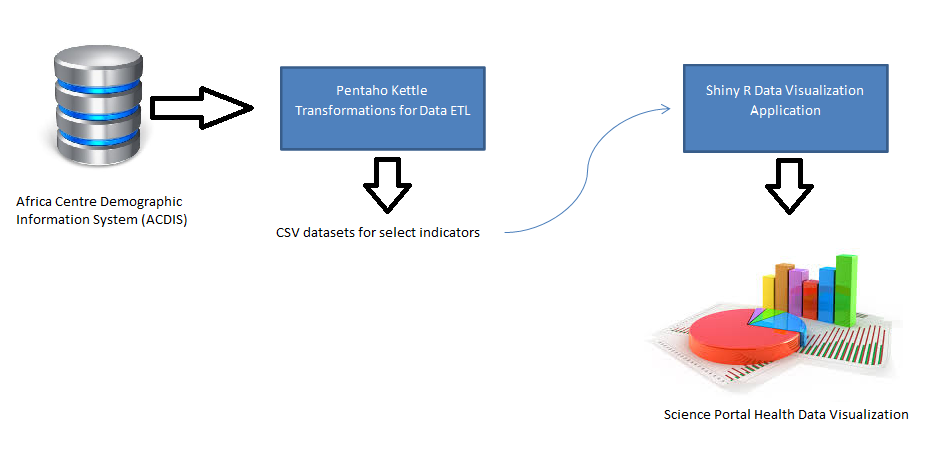
\includegraphics[scale=0.4]{./Chapter4/images/scienceportaloverview}% [width=6in, height=4in]{our}
\caption{Overview of Scientific Portal solution }
\label{fig1}
\end{figure}

\subsection{Data Operations Portal}
The Data Operations Portal screen is placed within the Data Centre. This is the office which deals with data collection, data entry, data cleaning, data quality assurance and data archiving. This will be a dashboard which aims to give real-time feedback on the progress of data collection activities, data entry activities and data archiving activities measured against the total number of data forms allocated for a particular survey round of three studies; Household, Individual and Verbal Autopsy. This is in order to keep the Data Centre team abreast of their progress and operational bottlenecks in a transparent and accessible manner.

For this portal, data will be pulled directly from a Microsoft SQL Server via polling for changes in the underlying data every hour.
This portal is not be externally accessible as it is purely for operational monitoring.

\begin{figure}[!ht] 
\centering
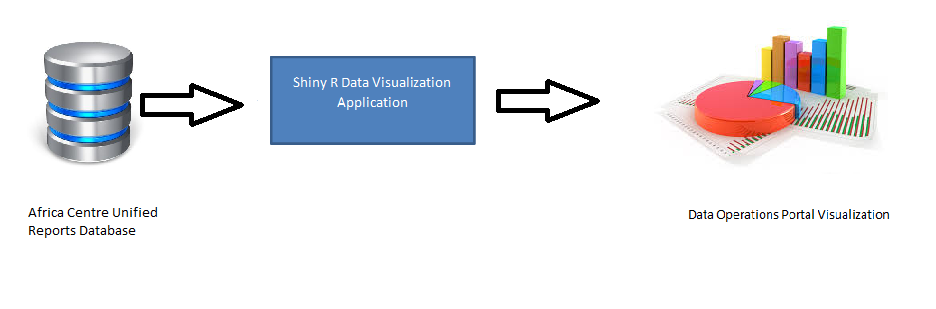
\includegraphics[scale=0.4]{./Chapter4/images/operationsportaloverview}
\caption{Overview of Data Operations Portal solution }
\label{fig2}
\end{figure}

\subsection{Community Engagement Portal}

The third and final screen is strategically placed in the Africa Centre foyer, visible and accessible to both staff and visitors. Its main focus is to package data which is of interest to the community which Africa Centre’s research serves into visual representations that are easy to interpret. This portal can be externally accessible over the internet for the community at large to access.

\begin{figure}[!ht] 
\centering
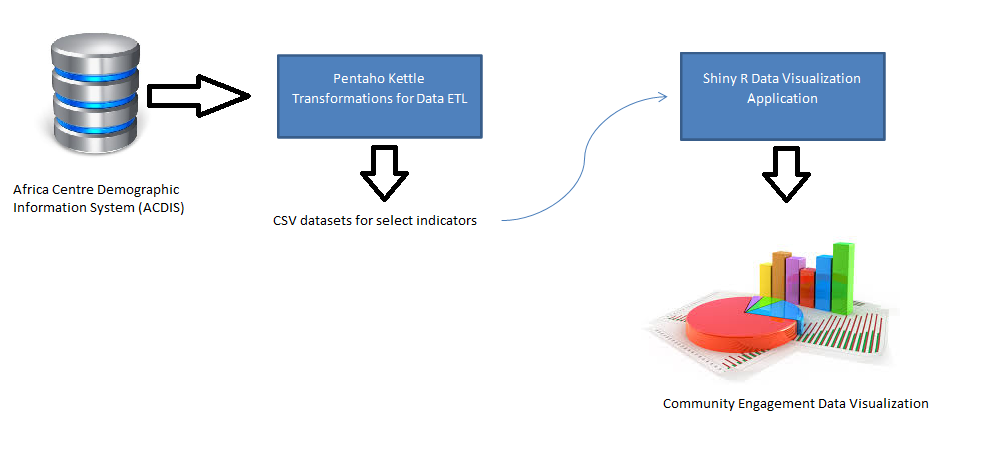
\includegraphics[scale=0.4]{./Chapter4/images/communityportaloverview}
\caption{Overview of Community Engagement Portal solution }
\label{fig3}
\end{figure}

This research is about creating a generalizable data visualization solution for INDEPTH HDSS sites, and the output will be a software application which can visualize data at any of these sites. Different sites have differing data cleaning and data manipulation strategies and as such, the onus of ensuring that the data fed into the visualization platform is clean and has handled missing data falls on the data manager at the site. The only constant in the provided solution will be the software application; the ETL transformations and jobs at each INDEPTH site will have to be developed by the site data managers to handle each HDSS sites’ database idiosyncrasies which are best known by the on site data manager. In order to do this, they will be informed by certain dataset structures and conventions which we have documented and are elaborated on in chapter 5
